% Full instructions available at:
% https://github.com/elauksap/focus-beamertheme

\documentclass{beamer}
\usetheme[numbering=progressbar]{focus}
\usepackage{tikz}
\usetikzlibrary{positioning}
\usetikzlibrary{shapes,arrows}
\usepackage{transparent}
\usepackage{fancyvrb}
\usepackage{listings}
\usepackage[utf8]{inputenc}
\definecolor{main}{RGB}{47, 161, 219}
%\definecolor{textcolor}{RGB}{128, 128, 128}
\definecolor{background}{RGB}{240, 247, 255}
\definecolor{textcolor}{RGB}{85, 87, 83}
\title{D4 Project}
\subtitle{Open and collaborative network monitoring}
\author{Aurélien Thirion, Jean-Louis Huynen}
\titlegraphic{\includegraphics[scale=0.20]{d4-logo.pdf}}
\institute{Team CIRCL \\ \url{https://www.d4-project.org/}}
\date{20190307}

\begin{document}
    \begin{frame}
        \maketitle
    \end{frame}

\begin{frame}
        \frametitle{Problem statement}
        \begin{itemize}
                \item CSIRTs (or private organisations) build their {\bf own honeypot, honeynet or blackhole monitoring network}
                \item Designing, managing and operating such infrastructure is a tedious and resource intensive task
                \item {\bf Automatic sharing} between monitoring networks from different organisations is missing
                \item Sensors and processing are often seen as blackbox or difficult to audit

        \end{itemize}
\end{frame}


\begin{frame}
 \frametitle{Objective}
 \begin{itemize}
         \item Based on our experience with MISP\footnote{\url{https://github.com/MISP/MISP}} where sharing played an important role, we transpose
                 the model in D4 project
         \item Keeping the protocol and code base {\bf simple and minimal}
         \item Allowing every organisation to {\bf control and audit their own sensor network}
         \item Extending D4 or {\bf encapsulating legacy monitoring protocols} must be as simple as possible
         \item Ensuring that the sensor server has {\bf no control on the sensor} (unidirectional streaming)
         \item Don't force users to use dedicated sensors and allow {\bf flexibility of sensor support} (software, hardware, virtual)

 \end{itemize}
\end{frame}

\begin{frame}
        \frametitle{(short) History}
 \begin{itemize}
        \item D4 Project (co-funded under INEA CEF EU program) started - 1st November 2018
        \item D4 encapsulation protocol version 1 published  - 1st December 2018
        \item v0.1 release of the D4 core\footnote{\url{https://www.github.com/D4-project/d4-core}} including a server and simple D4 C client - 21st January 2018
        \item First version of a golang D4 client\footnote{\url{https://www.github.com/D4-project/d4-goclient/}} running on ARM, MIPS, PPC and x86 - January 2018
 \end{itemize}
\end{frame}

\begin{frame}
\frametitle{D4 Overview}
        \includegraphics[scale=0.41]{d4-overview.pdf}
\end{frame}

\begin{frame}
        \frametitle{Roadmap (next 2 months)}
        \begin{itemize}
                \item Passive DNS analyzer (alpha version released)
                \item Passive SSL collector and analyzer
                \item Backscatter DDoS traffic analyzer
                \item {\bf Default server} (blackhole monitoring or Passive DNS collector) at CIRCL for organisations willing to contribute without running their own D4 server
        \end{itemize}
\end{frame}


\begin{frame}
        \frametitle{D4 encapsulation protocol}
        \includegraphics[scale=0.38]{d4-protocol-encapsulation.png}
\end{frame}

\begin{frame}
        \frametitle{D4 server - main interface}
        \includegraphics[scale=0.18]{d4-4.png}
\end{frame}

\begin{frame}
        \frametitle{D4 server - server management}
        \includegraphics[scale=0.18]{d4-3.png}
\end{frame}

\begin{frame}
        \frametitle{D4 server - sensor overview}
        \includegraphics[scale=0.18]{d4-1.png}
\end{frame}


\begin{frame}
        \frametitle{D4 server - sensor management}
        \includegraphics[scale=0.18]{d4-2.png}
\end{frame}


\begin{frame}
        \frametitle{D4 client example : A passive SSL fingerprinter}
        \begin{columns}
            \begin{column}{0.5\textwidth}
              \begin{center}
                \includegraphics[scale=0.2]{monitor.png}
              \end{center}
            \end{column}
            \begin{column}{0.5\textwidth} 
              \begin{center}
                \includegraphics[scale=0.2]{orangepi.png}
              \end{center}
            \end{column}
          \end{columns}
          \hspace{20pt}
          \begin{itemize}
            \item 1 desktop monitored during 15 days
            \item 3327 TLS sessions fingerprinted
            \item 600 unique certificates collected
          \end{itemize}
\end{frame}

\begin{frame}
\frametitle{Get in touch if you want to join the project, host a sensor or contribute}
\begin{itemize}
\item Collaboration can include research partnership, sharing of collected streams or improving the software.
\item Contact: info@circl.lu
\item \url{https://github.com/D4-Project} -  \url{https://twitter.com/d4_project}
\end{itemize}
\end{frame}

\end{document}
